% !TEX TS-program = pdflatex
% !TEX encoding = UTF-8 Unicode

% This is a simple template for a LaTeX document using the "article" class.
% See "book", "report", "letter" for other types of document.

\documentclass[12pt]{article}
\usepackage[round, sort , authoryear]{natbib}
\usepackage[T1]{fontenc}
%%% PAGE DIMENSIONS
\usepackage[margin=2.5 cm]{geometry}
\usepackage{blindtext} % to change the page dimensions
\geometry{a4paper} % or letterpaper (US) or a5paper or....
% \geometry{margin=2in} % for example, change the margins to 2 inches all round
% \geometry{landscape} % set up the page for landscape
%   read geometry.pdf for detailed page layout information
\usepackage[utf8]{inputenc} 
\usepackage{graphicx} % support the \includegraphics command and options
\usepackage{epstopdf}
% \usepackage[parfill]{parskip} % Activate to begin paragraphs with an empty line rather than an indent
\usepackage{pgfplots}
\pgfplotsset{compat=1.13}
\usepackage{caption,fixltx2e}
\usepackage[flushleft]{threeparttable}
\usepackage{color, colortbl}
\definecolor{Gray}{gray}{0.9}
%%% PACKAGES
\usepackage{placeins}
\usepackage{booktabs} % for much better looking tables
\usepackage{array} % for better arrays (eg matrices) in maths
\usepackage{paralist} % very flexible & customisable lists (eg. enumerate/itemize, etc.)
\usepackage{verbatim} % adds environment for commenting out blocks of text & for better verbatim
% These packages are all incorporated in the memoir class to one degree or another...
\usepackage{amsmath}
\usepackage{cases}
\usepackage{graphicx}
\usepackage{float}
\usepackage{authblk}
\usepackage{pgfplots}
\usepackage{pdfpages}
\linespread{1.5}

\usepackage{amssymb} 
\usepackage{tabularx}
\usepackage{booktabs}   % for nice tables
\usepackage[colorlinks=false, linktocpage=true]{hyperref}


\usepackage{subcaption}
\usepackage{graphicx}

\captionsetup[sub]{labelformat=simple}

\newtheorem{assumption*}{\assumptionnumber}
\providecommand{\assumptionnumber}{}
\makeatletter
\newenvironment{assumption}[2]
{%
	\renewcommand{\assumptionnumber}{Assumption}%
	\begin{assumption*}%
		\protected@edef\@currentlabel{}%
	}
	{%
	\end{assumption*}
}
\makeatother
\hypersetup{
	colorlinks,
	linkcolor={red!50!black},
	citecolor={blue!50!black},
	urlcolor={blue!80!black}
}
% use for hypertext
\usepackage[colorinlistoftodos]{todonotes}

%For Figures, below

\usepackage{tikz}
\usetikzlibrary{shapes}
\usepgflibrary{arrows} % LATEX and plain TEX and pure pgf
\usepgflibrary[arrows] % ConTEXt and pure pgf
\usetikzlibrary{arrows} % LATEX and plain TEX when using Tik Z
\usetikzlibrary[arrows] % ConTEXt when using Tik Z
\usepackage{hyperref}
\def\sym#1{\ifmmode^{#1}\else\(^{#1}\)\fi}
\usepackage{booktabs}
\newcommand{\tabnotes}[2]{\bottomrule \multicolumn{#1}{@{}p{0.70\linewidth}@{}}{\footnotesize #2 }}

%%% The "real" document content comes below...
\title{Tables and Figures- Cohabitation and Divorce laws.}
\author{}

 \begin{document}
 	 % Bibliography style, important for biblatex functioning	
 	 \bibliographystyle{apa}
 	 
 	\maketitle
 	
 	\section{Wealth regression}
 	
 	\begin{table}[H]\centering                                  \scriptsize                                 \caption{Changes in net worth upon divorce and breakup}                                   \label{tab:assdiv}                                 \resizebox{0.8\textwidth}{!}{                                 \begin{tabular}{l*{2}{c}} \toprule                             \textit{Dependent variable:}&\multicolumn{2}{c}{Inividual net worth after divorce/breakup}\\                                 \textit{Sample:}& Divorces & Breakups  \\
\midrule
Current total household income&      0.1918\sym{***}&      0.1223\sym{***}\\
                    &    (0.0636)         &    (0.0459)         \\
[1em]
Couple's net worth before divorce/breakup&      0.3848\sym{***}&      0.4947\sym{***}\\
                    &    (0.0094)         &    (0.0120)         \\
[1em]
Constant            &     -0.4050         &     -0.2274         \\
                    &    (0.3255)         &    (0.2044)         \\
\hline
Dependent variable mean&       6.281         &       3.604         \\
Observations        &        1084         &         646         \\
\bottomrule
\noalign{\smallskip}
\end{tabular}
}
\begin{minipage}{\textwidth}
\scriptsize\smallskip
Results from median regressions, a particular instance of the median regression, using data from the 1999-2019 PSID. The sample includes household head (men or women) who experienced a divorce or a breakup in the two years before the interview. We regress their individual net worth after the breakup on the couple's net worth before the breakup. Net worth and income are expressed in 1997 10,000 dollars. Coefficients that are significantly different from zero are denoted by *10\%, **5\%, and ***1\%.
\\
\end{minipage}
\end{table}

 \section{Partnership choice}


\begin{table}[!htbp]\centering
	\caption{\\Descriptive statistics, relationship sample}
	\label{table:sum_rel}
	{
\def\sym#1{\ifmmode^{#1}\else\(^{#1}\)\fi}
\begin{tabular}{l*{1}{cccc}}
\toprule
                    &           N&        Mean&      Median&          SD\\
\midrule
Marry (0/1)         &       11292&        0.73&           1&        0.45\\
Cohabit (0/1)       &       11292&        0.27&           0&        0.45\\
College (0/1)       &       11292&        0.20&           0&        0.40\\
Year the Cohabitation began&       11202&     1970.93&        1972&       10.08\\
Unilateral divorce when relationship began (0/1)&       11292&        0.30&           0&        0.46\\
Age of respondent   &       11292&       39.89&          38&       12.17\\
\bottomrule
\end{tabular}
}

\end{table}
\FloatBarrier

%\begin{table}[H]\centering                                  \scriptsize                                 \caption{The average effect of unilateral divorce on the choice between cohabitation and marriage among newly formed couples}                                   \label{tab:tabrel}                                 \resizebox{0.8\textwidth}{!}{                                 \begin{tabular}{l*{4}{c}} \toprule                                 &\multicolumn{4}{c}{\textit{Dependent variable: marry (1), cohabit (0)} }\\
\midrule
Unilateral          &     -0.0917\sym{***}&     -0.0836\sym{***}&     -0.0846\sym{***}&     -0.0778\sym{***}\\
                    &    (0.0249)         &    (0.0237)         &    (0.0302)         &    (0.0295)         \\
State FE     & Yes & Yes& Yes & Yes\\                       Period relationship began FE     & Yes & Yes& Yes & Yes\\                           Additional controls    & No & Yes& No& Yes\\                                           State-specific linear time trend    & No & No & Yes & Yes\\
Dependent variable mean&       0.725         &       0.725         &       0.725         &       0.725         \\
Observations        &       11165         &       11165         &       11165         &       11165         \\
\bottomrule
\noalign{\smallskip}
\end{tabular}
}
\begin{minipage}{\textwidth}
\scriptsize\smallskip
Notes: This table reports the average effect of unilateral divorce on the choice between cohabitation and marriage. The analysis follows the methodology outlined in \cite{borusyak2021} uses and the \textit{relationships sample}. The unit of observation refers to newly formed couples (either married or cohabiting) in state \textit{s} and year \textit{t}. The dummy variable \textit{Unilateral Divorce} takes the value 1 if unilateral divorce was in effect in state \textit{s} and year \textit{t} and 0 otherwise. The additional controls include dummies for ethnicity, age, and education. Standard errors are clustered at the state level. Coefficients that are significantly different from zero are denoted by *10\%, **5\%, and ***1\%.
\\
\end{minipage}\vspace{-6mm}
\end{table}


 \begin{figure}
	\centering
	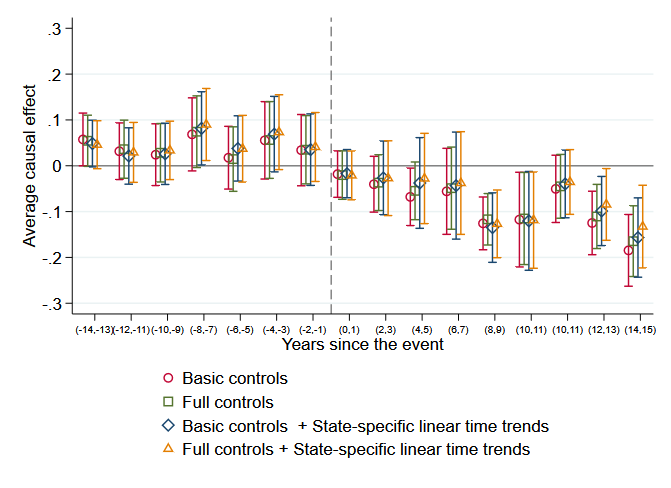
\includegraphics[width=0.7\linewidth]{C:/Users/Fabio/Dropbox/py_mar_3/Analysis/output/event_graph_rel}
	\caption{}
	\label{fig:eventgraphrel}
\end{figure}


%\begin{figure}[H]
%	\caption{\\Event studies of cohabitation duration around the introduction of unilateral divorce}
%	\label{fig:rsd}
%	\begin{subfigure}{.49\textwidth}
%		\centering
%		\caption{Basic controls}
%		\label{fig:rsd_bc}
%		\includegraphics[width=\textwidth]{C:/Users/Fabio/Dropbox/py_mar_3/Analysis/output/event_graph_rel1.png}
%	\end{subfigure}
%	\begin{subfigure}{.49\textwidth}
%		\centering
%		\caption{Full controls}
%		\label{fig:rsd_fc}
%		\includegraphics[width=\textwidth]{C:/Users/Fabio/Dropbox/py_mar_3/Analysis/output/event_graph_rel2.png}
%	\end{subfigure}
	
	
%	\hspace{20em}
	
%	\begin{subfigure}{.49\textwidth}
%		\centering
%		\caption{Basic controls+linear time trend by State}
%		\label{fig:rsd_bct}
%		\includegraphics[width=\textwidth]{C:/Users/Fabio/Dropbox/py_mar_3/Analysis/output/event_graph_rel3.png}
%	\end{subfigure}
%	\begin{subfigure}{.49\textwidth}
%		\centering
%		\caption{Full controls+linear time trend by State}
%		\label{fig:rsd_fct}
%		\includegraphics[width=\textwidth]{C:/Users/Fabio/Dropbox/py_mar_3/Analysis/output/event_graph_rel4.png}
%	\end{subfigure}
%\end{figure}
%\FloatBarrier


\begin{table}[H]\centering                                  \scriptsize                                  \caption{The average effect of unilateral divorce on the choice between cohabitation and marriage among newly formed couples, by property regime upon divorce}                    \label{tab:tabrelcom}                                 \resizebox{0.8\textwidth}{!}{                                 \begin{tabular}{l*{4}{c}} \toprule                                 &\multicolumn{4}{c}{\textit{Dependent variable: marry (1), cohabit (0)}}\\                                 \textit{Sample:}& ComP & ComP &  Tit & Tit \\
\midrule
Unilateral          &     -0.1345\sym{***}&     -0.1327\sym{***}&     -0.0637\sym{*}  &     -0.0573\sym{*}  \\
                    &    (0.0507)         &    (0.0451)         &    (0.0332)         &    (0.0325)         \\
State FE     & Yes & Yes& Yes & Yes\\                       Period relationship began FE     & Yes & Yes& Yes & Yes\\                           Additional controls    & No & Yes& No& Yes\\
Dependent variable mean&       0.685         &       0.685         &       0.806         &       0.806         \\
Observations        &        2324         &        2324         &        4631         &        4631         \\
\bottomrule
\noalign{\smallskip}
\end{tabular}
}
\begin{minipage}{\textwidth}
\scriptsize\smallskip
Notes: This table reports the average effect of unilateral divorce on the choice between cohabitation and marriage. The analysis follows the methodology outlined in \cite{borusyak2021} uses and the \textit{relationships sample}. The unit of observation refers to newly formed couples (either married or cohabiting) in state \textit{s} and year \textit{t}. The dummy variable \textit{Unilateral Divorce} takes the value 1 if unilateral divorce was in effect in state \textit{s} and year \textit{t} and 0 otherwise. The additional controls include dummies for ethnicity, age, and education. ComP: community property states; Tit: title based regime. Standard errors are clustered at the state level. Coefficients that are significantly different from zero are denoted by *10\%, **5\%, and ***1\%.
\\
\end{minipage}
\end{table}


\begin{table}[H]\centering                                  \scriptsize                                                                  \caption{The average effect of unilateral divorce on the choice between cohabitation and marriage among newly formed couples, by the presence of children}                                   \label{tab:tabrelch}                                 \resizebox{0.8\textwidth}{!}{                                 \begin{tabular}{l*{2}{c}} \toprule                                 &\multicolumn{2}{c}{\textit{Dependent variable: marry (1), cohabit (0)}}\\                                 \textit{Sample:}& Some children &  Childless \\
\midrule
Unilateral          &     -0.0661\sym{***}&     -0.1044\sym{**} \\
                    &    (0.0234)         &    (0.0410)         \\
State FE     & Yes & Yes \\                       Period relationship began FE     & Yes & Yes \\                           Additional controls    & Yes & Yes\\
Dependent variable mean&       0.771         &       0.534         \\
Observations        &        8875         &        2269         \\
\bottomrule
\noalign{\smallskip}
\end{tabular}
}
\begin{minipage}{\textwidth}
\scriptsize\smallskip
Notes: This table reports the average effect of unilateral divorce on the choice between cohabitation and marriage. The analysis follows the methodology outlined in \cite{borusyak2021} uses and the \textit{relationships sample}. The unit of observation refers to newly formed couples (either married or cohabiting) in state \textit{s} and year \textit{t}. The dummy variable \textit{Unilateral Divorce} takes the value 1 if unilateral divorce was in effect in state \textit{s} and year \textit{t} and 0 otherwise. The additional controls include dummies for ethnicity, age, and education. Standard errors are clustered at the state level. Coefficients that are significantly different from zero are denoted by *10\%, **5\%, and ***1\%.
\\
\end{minipage}
\end{table}



\begin{table}[H]\centering                                  \scriptsize                                                                  \caption{The average effect of unilateral divorce on the choice of cohabitation vs. marriage among newly formed couples. Sample of never movers}                                   \label{tab:tabrelkeep}                                 \resizebox{0.8\textwidth}{!}{                                 \begin{tabular}{l*{4}{c}} \toprule                                 &\multicolumn{4}{c}{\textit{Dependent variable: marry (1), cohabit (0)}}\\
\midrule
Unilateral          &     -0.0928\sym{***}&     -0.0881\sym{***}&     -0.0865\sym{***}&     -0.0842\sym{**} \\
                    &    (0.0278)         &    (0.0273)         &    (0.0322)         &    (0.0335)         \\
State FE     & Yes & Yes& Yes & Yes\\                       Period relationship began FE     & Yes & Yes& Yes & Yes\\                           Additional controls    & No & Yes& No& Yes\\                                           State-specific linear time trend    & No & No & Yes & Yes\\
Dependent variable mean&       0.734         &       0.734         &       0.734         &       0.734         \\
Observations        &        7798         &        7798         &        7798         &        7798         \\
\bottomrule
\noalign{\smallskip}
\end{tabular}
}
\begin{minipage}{\textwidth}
\scriptsize\smallskip
Notes: This table reports the average effect of unilateral divorce on the choice between cohabitation and marriage. The analysis follows the methodology outlined in \cite{borusyak2021} uses and the \textit{relationships sample}. The sample used for this regression includes only respondents who still live in the same state where they were living at sixteen years old. The unit of observation refers to newly formed couples (either married or cohabiting) in state \textit{s} and year \textit{t}. The dummy variable \textit{Unilateral Divorce} takes the value 1 if unilateral divorce was in effect in state \textit{s} and year \textit{t} and 0 otherwise. The additional controls include dummies for ethnicity, age, and education. Standard errors are clustered at the state level. Coefficients that are significantly different from zero are denoted by *10\%, **5\%, and ***1\%.
\\
\end{minipage}
\end{table}



\begin{table}[H]\centering                                                                   \caption{The average effect of unilateral divorce on the choice of cohabitation vs. marriage vs. staying single for single individuals}                                   \label{tab:tabrel}                                 \resizebox{\textwidth}{!}{                                 \begin{tabular}{@{\extracolsep{4pt}}lcccc} \toprule                                  &\multicolumn{2}{c}{\textit{Dependent variable: marry (1), stay single (0) }}&\multicolumn{2}{c}{\textit{Dependent variable: cohabit (1), stay single (0)}}\\
\cline{2-3}\cline{4-5}
Unilateral Divorce  &     -0.0033         &     -0.0056         &      0.0114\sym{***}&      0.0137\sym{***}\\
                    &    (0.0037)         &    (0.0059)         &    (0.0021)         &    (0.0034)         \\
State FE     & Yes & Yes& Yes & Yes\\                       Year FE     & Yes & Yes& Yes & Yes\\                           Additional controls    & No & Yes& No& Yes\\
Dependent variable mean&       0.075         &       0.098         &       0.024         &       0.032         \\
Observations        &       78512         &       60535         &       78512         &       60535         \\
\bottomrule
\noalign{\smallskip}
\end{tabular}
}
\begin{minipage}{\textwidth}
\scriptsize\smallskip
Notes: This table reports the average effect of unilateral divorce on the choice of cohabitation vs. marriage vs. staying single using the methodology of \cite{borusyak2021} and data from the the \textit{relationships sample}. The unit of observation is one person-month where the respondent was single. Depending on the spefication, we study the risk of marriage (brekup) of singleness spells, where the event of breakup (marriage) is treated as censoring. The dummy variable \textit{Unilateral Divorce} takes value 1 if unilateral divorce was in place in state \textit{s} and year \textit{t} and 0 otherwise. The additional controls include dummies for ethnicity, age, education, and duration of the singleness spell. Standard errors are clustered at the state level. Coefficients that are significantly different from zero are denoted by *10\%, **5\%, and ***1\%.
\\
\end{minipage}
\end{table}


%\input{C:/Users/Fabio/Dropbox/py_mar_3/Analysis/output/reg_rel_nsfg}
 \section{Cohabitation duration.}
 

\begin{table}[!htbp]\centering
	\caption{\\Descriptive statistics, cohabitation sample}
	\label{table:sum_coh}
	{
\def\sym#1{\ifmmode^{#1}\else\(^{#1}\)\fi}
\begin{tabular}{l*{1}{cccc}}
\toprule
                    &           N&        Mean&      Median&          SD\\
\midrule
End of Cohabitation spell: Censored (0/1)&        4581&        0.31&           0&        0.46\\
End of Cohabitation spell: Marry (0/1)&        4581&        0.56&           1&        0.50\\
End of Cohabitation spell: Breakup (0/1)&        4581&        0.13&           0&        0.34\\
College (0/1)       &        4581&        0.18&           0&        0.39\\
Length of Cohabitation (months)&        4581&       22.45&          13&       29.07\\
Year the Cohabitation began&        4581&     1978.12&        1979&        7.11\\
Unilateral divorce when Cohabitation began (0/1)&        4581&        0.49&           0&        0.50\\
Age of respondent   &        4581&       34.44&          33&       10.08\\
\bottomrule
\end{tabular}
}

\end{table} 
 
 \begin{table}[H]\centering                                  \scriptsize                                 \caption{The average effect of unilateral divorce on the probability that cohabitation ends in breakup vs. marriage. Unit of observation: end of a cohabitation spell}                                   \label{tab:tabsep}                                 \resizebox{0.8\textwidth}{!}{                                 \begin{tabular}{l*{4}{c}} \toprule                             &\multicolumn{4}{c}{\textit{Dependent variable: marry (0), breakup (1)}}\\
\midrule
Unilateral          &     -0.0037         &     -0.0169         &      0.0563         &      0.0486         \\
                    &    (0.0338)         &    (0.0313)         &    (0.0766)         &    (0.0698)         \\
State FE     & Yes & Yes& Yes & Yes\\                       Year cohabitation began FE     & Yes & Yes& Yes & Yes\\                           Additional controls    & No & Yes& No& Yes\\                                           State-specific linear time trend    & No & No & Yes & Yes\\
Dependent variable mean&       0.379         &       0.379         &       0.354         &       0.354         \\
Observations        &        3852         &        3852         &      105384         &      105384         \\
\bottomrule
\noalign{\smallskip}
\end{tabular}
}
\begin{minipage}{\textwidth}
\scriptsize\smallskip
Notes: This table reports the average effect of unilateral divorce on the probability of cohabitation ending in a breakup vs. marriage. The analysis follows the methodology outlined in \cite{borusyak2021} uses and the \textit{cohabitations sample}. The unit of observation is the end of a cohabitation spell (either marriage or breakup) which \textit{started} in state \textit{s} and year \textit{t}. The dummy variable \textit{Unilateral Divorce} takes value 1 if unilateral divorce was in effect in state \textit{s} and year \textit{t}. The additional controls include dummies for ethnicity, age, and education. The sample associated to regressions including State-specific linear time trend excludes five states due to multicollinearity. Standard errors are clustered at the state level. Coefficients that are significantly different from zero are denoted by *10\%, **5\%, and ***1\%.
\\
\end{minipage}
\end{table}

 
 

\begin{table}[H]\centering                                  \scriptsize                                 \caption{The average effect of unilateral divorce on the probability that a cohabitation spell ends (because of marriage or breakup). Unit of observation: cohabitation-month}                                   \label{tab:tabdur}                                 \resizebox{0.8\textwidth}{!}{                                 \begin{tabular}{l*{4}{c}} \toprule                                 \textit{Dependent variable:}&\multicolumn{4}{c}{\textit{keep cohabiting (0), cohabitation ends (1)}}\\
\midrule
Unilateral          &     -0.0162\sym{***}&     -0.0131\sym{***}&     -0.0191\sym{***}&     -0.0149\sym{**} \\
                    &    (0.0048)         &    (0.0046)         &    (0.0061)         &    (0.0059)         \\
State FE     & Yes & Yes& Yes & Yes\\                       Year cohabitation began FE     & Yes & Yes& Yes & Yes\\                           Additional controls    & No & Yes& No& Yes\\                                           State-specific linear time trend    & No & No & Yes & Yes\\
Dependent variable mean&       0.037         &       0.037         &       0.037         &       0.037         \\
Observations        &      105384         &      105384         &      105384         &      105384         \\
\bottomrule
\noalign{\smallskip}
\end{tabular}
}
\begin{minipage}{\textwidth}
\scriptsize\smallskip
Notes: This table reports the average effect of unilateral divorce on the probability of cohabitation ending in a breakup or marriage. The analysis follows the methodology outlined in \cite{borusyak2021} uses and the \textit{cohabitations sample}. The unit of observation is one cohabitation-month, which corresponds to a specific month within a particular cohabitation spell. The focus of this table is to report the probability of a cohabitation spell (initiated in state \textit{s} and year \textit{t}) ending in a breakup or marriage. The dummy variable \textit{Unilateral Divorce} takes value 1 if unilateral divorce was in effect in state \textit{s} and year \textit{t} at the start of the cohabitation spell. The additional controls include dummies for ethnicity, age, education, duration of cohabitation, and the introduction of unilateral divorce \textit{after} the cohabitation period commenced. Standard errors are clustered at the state level. Coefficients that are significantly different from zero are denoted by *10\%, **5\%, and ***1\%.
\\
\end{minipage}
\end{table}

 
  \begin{figure}
 	\centering
 	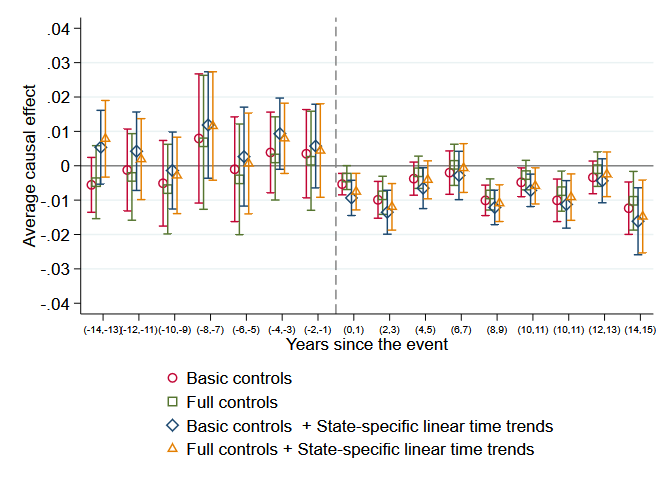
\includegraphics[width=0.7\linewidth]{C:/Users/Fabio/Dropbox/py_mar_3/Analysis/output/event_graph_dur}
 	\caption{}
 	\label{fig:eventgraphdur}
 \end{figure}


%\begin{figure}[H]
%	\caption{\\Event studies of cohabitation duration around the introduction of unilateral divorce}
%	\label{fig:esd}
%		\begin{subfigure}{.49\textwidth}
%			\centering
%			\caption{Basic controls}
%			\label{fig:esd_bc}
%			\includegraphics[width=\textwidth]{C:/Users/Fabio/Dropbox/py_mar_3/Analysis/output/event_graph_dur1.png}
%		\end{subfigure}
%		\begin{subfigure}{.49\textwidth}
%			\centering
%			\caption{Full controls}
%			\label{fig:esd_fc}
%			\includegraphics[width=\textwidth]{C:/Users/Fabio/Dropbox/py_mar_3/Analysis/output/event_graph_dur2.png}
%		\end{subfigure}

	
	\hspace{20em}
	
	


 \begin{table}[H]\centering                                  \scriptsize                                 \caption{The average effect of unilateral divorce on the probability that a cohabitation spell ends in a breakup. Unit of observation: cohabitation-month}                                   \label{tab:tabdurb}                                 \resizebox{0.8\textwidth}{!}{                                 \begin{tabular}{l*{4}{c}} \toprule                                 &\multicolumn{4}{c}{\textit{Dependent variable: keep cohabiting (0), breakup (1)}}\\
\midrule
Unilateral          &     -0.0068\sym{***}&     -0.0044\sym{**} &     -0.0105\sym{***}&     -0.0085\sym{***}\\
                    &    (0.0016)         &    (0.0018)         &    (0.0021)         &    (0.0023)         \\
State FE     & Yes & Yes& Yes & Yes\\                       Year cohabitation began FE     & Yes & Yes& Yes & Yes\\                           Additional controls    & No & Yes& No& Yes\\                                           State-specific linear time trend    & No & No & Yes & Yes\\
Dependent variable mean&       0.014         &       0.014         &       0.014         &       0.014         \\
Observations        &      105384         &      105384         &      105384         &      105384         \\
\bottomrule
\noalign{\smallskip}
\end{tabular}
}
\begin{minipage}{\textwidth}
\scriptsize\smallskip
Notes: This table reports the average effect of unilateral divorce on the probability of cohabitation ending in a breakup. The analysis follows the methodology outlined in \cite{borusyak2021} uses and the \textit{cohabitations sample}. The unit of observation is one cohabitation-month, which corresponds to a specific month within a particular cohabitation spell. The focus of this table is to report the probability of a cohabitation spell (initiated in state \textit{s} and year \textit{t}) ending in a breakup, with the occurrence of marriage considered as a termination point (right censoring) for the cohabitation period. The dummy variable \textit{Unilateral Divorce} takes value 1 if unilateral divorce was in effect in state \textit{s} and year \textit{t} at the start of the cohabitation spell. The additional controls include dummies for ethnicity, age, education duration of cohabitation, and the introduction of unilateral divorce \textit{after} the cohabitation period commenced. Standard errors are clustered at the state level. Coefficients that are significantly different from zero are denoted by *10\%, **5\%, and ***1\%.
\\
\end{minipage}\vspace{-6mm}
\end{table}

  \begin{table}[H]\centering                                  \scriptsize                                 \caption{The average effect of unilateral divorce on the probability that a cohabitation spell ends in a marriage. Unit of observation: cohabitation-month}                                   \label{tab:tabdurm}                                 \resizebox{0.8\textwidth}{!}{                                 \begin{tabular}{l*{4}{c}} \toprule                                 &\multicolumn{4}{c}{\textit{Dependent variable: keep cohabiting (0), marry (1)}}\\
\midrule
Unilateral          &     -0.0095\sym{**} &     -0.0087\sym{**} &     -0.0085\sym{*}  &     -0.0064         \\
                    &    (0.0041)         &    (0.0040)         &    (0.0051)         &    (0.0050)         \\
State FE     & Yes & Yes& Yes & Yes\\                       Year cohabitation began FE     & Yes & Yes& Yes & Yes\\                           Additional controls    & No & Yes& No& Yes\\                                           State-specific linear time trend    & No & No & Yes & Yes\\
Dependent variable mean&       0.023         &       0.023         &       0.023         &       0.023         \\
Observations        &      105384         &      105384         &      105384         &      105384         \\
\bottomrule
\noalign{\smallskip}
\end{tabular}
}
\begin{minipage}{\textwidth}
\scriptsize\smallskip
Notes: This table reports the average effect of unilateral divorce on the probability of cohabitation ending in a marriage. The analysis follows the methodology outlined in \cite{borusyak2021} uses and the \textit{cohabitations sample}. The unit of observation is one cohabitation-month, which corresponds to a specific month within a particular cohabitation spell. The focus of this table is to report the probability of a cohabitation spell (initiated in state \textit{s} and year \textit{t}) ending in a marriage, with the occurrence of breakup considered as a termination point (right censoring) for the cohabitation period. The dummy variable \textit{Unilateral Divorce} takes value 1 if unilateral divorce was in effect in state \textit{s} and year \textit{t} at the start of the cohabitation spell. The additional controls include dummies for ethnicity, age, education, duration of cohabitation, and the introduction of unilateral divorce \textit{after} the cohabitation period commenced. Standard errors are clustered at the state level. Coefficients that are significantly different from zero are denoted by *10\%, **5\%, and ***1\%.
\\
\end{minipage}
\end{table}

 \begin{table}[H]\centering                                  \scriptsize                                 \caption{The average effect of unilateral divorce on the probability that a cohabitation spell ends in a breakup by property regime at divorce. Unit of observation: cohabitation-month}                                   \label{tab:tabdurbcom}                                 \resizebox{0.8\textwidth}{!}{                                 \begin{tabular}{l*{4}{c}} \toprule                                 &\multicolumn{4}{c}{\textit{Dependent variable: keep cohabiting (0), breakup (1)}}\\                                 \textit{Sample:}& ComP & ComP &  Tit & Tit \\
\midrule
Unilateral          &     -0.0140\sym{**} &     -0.0144\sym{**} &     -0.0001         &      0.0016         \\
                    &    (0.0059)         &    (0.0071)         &    (0.0028)         &    (0.0036)         \\
State FE     & Yes & Yes& Yes & Yes\\                       Year cohabitation began FE     & Yes & Yes& Yes & Yes\\                           Additional controls    & No & Yes& No& Yes\\
Dependent variable mean&       0.035         &       0.035         &       0.033         &       0.033         \\
Observations        &       25243         &       25243         &       34624         &       34624         \\
\bottomrule
\noalign{\smallskip}
\end{tabular}
}
\begin{minipage}{\textwidth}
\scriptsize\smallskip
Notes: This table reports the average effect of unilateral divorce on the probability of cohabitation ending in a breakup. The analysis follows the methodology outlined in \cite{borusyak2021} uses and the \textit{cohabitations sample}. The unit of observation is one cohabitation-month, which corresponds to a specific month within a particular cohabitation spell. The focus of this table is to report the probability of a cohabitation spell (initiated in state \textit{s} and year \textit{t}) ending in a breakup, with the occurrence of marriage considered as a termination point (right censoring) for the cohabitation period. The dummy variable \textit{Unilateral Divorce} takes value 1 if unilateral divorce was in effect in state \textit{s} and year \textit{t} at the start of the cohabitation spell. The additional controls include dummies for ethnicity, age, education, duration of cohabitation,  and the introduction of unilateral divorce \textit{after} the cohabitation period commenced. ComP: community property states; Tit: title based regime. Standard errors are clustered at the state level. Coefficients that are significantly different from zero are denoted by *10\%, **5\%, and ***1\%.
\\
\end{minipage}
\end{table}
 
 \begin{table}[H]\centering                                  \scriptsize                                 \caption{The average effect of unilateral divorce on the probability that a cohabitation spell ends in a marriage by property regime at divorce. Unit of observation: cohabitation-month}                                   \label{tab:tabdurmcom}                                 \resizebox{0.8\textwidth}{!}{                                 \begin{tabular}{l*{4}{c}} \toprule                                 &\multicolumn{4}{c}{\textit{Dependent variable: keep cohabiting (0), marry (1)}}\\                                 \textit{Sample:}& ComP & ComP &  Tit & Tit \\
\midrule
Unilateral          &     -0.0163\sym{*}  &     -0.0216\sym{**} &     -0.0173\sym{***}&     -0.0169\sym{***}\\
                    &    (0.0095)         &    (0.0106)         &    (0.0028)         &    (0.0035)         \\
State FE     & Yes & Yes& Yes & Yes\\                       Year cohabitation began FE     & Yes & Yes& Yes & Yes\\                           Additional controls    & No & Yes& No& Yes\\
Dependent variable mean&       0.035         &       0.035         &       0.033         &       0.033         \\
Observations        &       25243         &       25243         &       34624         &       34624         \\
\bottomrule
\noalign{\smallskip}
\end{tabular}
}
\begin{minipage}{\textwidth}
\scriptsize\smallskip
Notes: This table reports the average effect of unilateral divorce on the probability of cohabitation ending in a marriage. The analysis follows the methodology outlined in \cite{borusyak2021} uses and the \textit{cohabitations sample}. The unit of observation is one cohabitation-month, which corresponds to a specific month within a particular cohabitation spell. The focus of this table is to report the probability of a cohabitation spell (initiated in state \textit{s} and year \textit{t}) ending in a marriage, with the occurrence of breakup considered as a termination point (right censoring) for the cohabitation period. The dummy variable \textit{Unilateral Divorce} takes value 1 if unilateral divorce was in effect in state \textit{s} and year \textit{t} at the start of the cohabitation spell. The additional controls include dummies for ethnicity, age, education, duration of cohabitation, and the introduction of unilateral divorce \textit{after} the cohabitation period commenced. ComP: community property states; Tit: title based regime. Standard errors are clustered at the state level. Coefficients that are significantly different from zero are denoted by *10\%, **5\%, and ***1\%.
\\
\end{minipage}
\end{table}

 
   \begin{table}[H]\centering                                  \scriptsize                                 \caption{The average effect of unilateral divorce on the probability that a cohabitation spell ends in a breakup. Unit of observation: cohabitation-month. Sample of never movers}                                   \label{tab:tabdurbk}                                 \resizebox{0.8\textwidth}{!}{                                 \begin{tabular}{l*{4}{c}} \toprule                                 &\multicolumn{4}{c}{\textit{Dependent variable: keep cohabiting (0), breakup (1)}}\\
\midrule
Unilateral          &     -0.0339\sym{***}&     -0.0328\sym{***}&     -0.0366\sym{***}&     -0.0355\sym{***}\\
                    &    (0.0028)         &    (0.0036)         &    (0.0031)         &    (0.0036)         \\
State FE     & Yes & Yes& Yes & Yes\\                       Year cohabitation began FE     & Yes & Yes& Yes & Yes\\                           Additional controls    & No & Yes& No& Yes\\                                           State-specific linear time trend    & No & No & Yes & Yes\\
Dependent variable mean&       0.014         &       0.014         &       0.014         &       0.014         \\
Observations        &       72828         &       72828         &       72828         &       72828         \\
\bottomrule
\noalign{\smallskip}
\end{tabular}
}
\begin{minipage}{\textwidth}
\scriptsize\smallskip
Notes: This table reports the average effect of unilateral divorce on the probability of cohabitation ending in a breakup. The analysis follows the methodology outlined in \cite{borusyak2021} uses and the \textit{cohabitations sample}. The unit of observation is one cohabitation-month, which corresponds to a specific month within a particular cohabitation spell.  The sample used for this regression includes only respondents who still live in the same state where they were living at sixteen years old. The focus of this table is to report the probability of a cohabitation spell (initiated in state \textit{s} and year \textit{t}) ending in a breakup, with the occurrence of marriage considered as a termination point (right censoring) for the cohabitation period. The dummy variable \textit{Unilateral Divorce} takes value 1 if unilateral divorce was in effect in state \textit{s} and year \textit{t} at the start of the cohabitation spell. The additional controls include dummies for ethnicity, age, education, duration of cohabitation, and the introduction of unilateral divorce \textit{after} the cohabitation period commenced. Standard errors are clustered at the state level. Coefficients that are significantly different from zero are denoted by *10\%, **5\%, and ***1\%.
\\
\end{minipage}
\end{table}

 \begin{table}[H]\centering                                  \scriptsize                                 \caption{The average effect of unilateral divorce on the probability that a cohabitation spell ends in a marriage. Unit of observation: cohabitation-month. Sample of never movers}                                   \label{tab:tabdurmk}                                 \resizebox{0.8\textwidth}{!}{                                 \begin{tabular}{l*{4}{c}} \toprule                                 &\multicolumn{4}{c}{\textit{Dependent variable: keep cohabiting (0), marry (1)}}\\
\midrule
Unilateral          &     -0.0175\sym{**} &     -0.0156\sym{**} &     -0.0210\sym{**} &     -0.0162\sym{**} \\
                    &    (0.0079)         &    (0.0071)         &    (0.0083)         &    (0.0071)         \\
State FE     & Yes & Yes& Yes & Yes\\                       Year cohabitation began FE     & Yes & Yes& Yes & Yes\\                           Additional controls    & No & Yes& No& Yes\\                                           State-specific linear time trend    & No & No & Yes & Yes\\
Dependent variable mean&       0.022         &       0.022         &       0.022         &       0.022         \\
Observations        &       72828         &       72828         &       72828         &       72828         \\
\bottomrule
\noalign{\smallskip}
\end{tabular}
}
\begin{minipage}{\textwidth}
\scriptsize\smallskip
Notes: This table reports the average effect of unilateral divorce on the probability of cohabitation ending in a marriage. The analysis follows the methodology outlined in \cite{borusyak2021} uses and the \textit{cohabitations sample}. The unit of observation is one cohabitation-month, which corresponds to a specific month within a particular cohabitation spell.  The sample used for this regression includes only respondents who still live in the same state where they were living at sixteen years old. The focus of this table is to report the probability of a cohabitation spell (initiated in state \textit{s} and year \textit{t}) ending in a marriage, with the occurrence of breakup considered as a termination point (right censoring) for the cohabitation period. The dummy variable \textit{Unilateral Divorce} takes value 1 if unilateral divorce was in effect in state \textit{s} and year \textit{t} at the start of the cohabitation spell. The additional controls include dummies for ethnicity, age, education, duration of cohabitation, and the introduction of unilateral divorce \textit{after} the cohabitation period commenced. Standard errors are clustered at the state level. Coefficients that are significantly different from zero are denoted by *10\%, **5\%, and ***1\%.
\\
\end{minipage}
\end{table}
 
 
% \input{C:/Users/Fabio/Dropbox/py_mar_3/Analysis/output/reg_sep_nsfg}
  %\input{C:/Users/Fabio/Dropbox/py_mar_3/Analysis/output/reg_dur_nsfg}
   
  \end{document}